% ============================================
% РАЗДЕЛ 3. РЕАЛИЗАЦИЯ И ЭКСПЕРИМЕНТАЛЬНАЯ АПРОБАЦИЯ
% ============================================

\section{Реализация системы и методика экспериментальной апробации}

В разделе~2 предложена каскадная архитектура из трёх ступеней,
обоснован выбор класса нейросетевого классификатора DS-CNN и
формализованы методы квантизации модели. Настоящий раздел
посвящён реализации описанной системы на платформе ESP32-S3,
методике систематического исследования архитектур
нейросетевого классификатора, разработке лабораторного
измерительного стенда, обеспечивающего регистрацию
энергопотребления с разрешением единиц микроампер, и методике
экспериментальной апробации. Изложение построено в той же
последовательности, что и работа системы: сначала рассматривается
реализация прошивки и тракта обработки звука, затем~--- методика
обучения и квантизации множества нейросетевых моделей,
далее~--- измерительная инфраструктура, и в завершение~---
методика эксперимента и формулы обработки полученных данных.

\subsection{Программная архитектура и реализация каскада}

\subsubsection{Конечный автомат каскада}

Логика работы каскадной системы реализована на платформе
ESP32-S3 в виде конечного автомата (Finite State Machine, FSM),
состояния которого соответствуют этапам цикла обработки,
описанным в разделе~2. Переходы между состояниями инициируются
либо аппаратными событиями (пробуждение по сигналу EXT1,
завершение DMA-передачи аудиоданных), либо программными
решениями (положительная классификация нейросетевой моделью,
истечение временно\'{г}о окна захвата). Состояния автомата
перечислены в таблице~\ref{tab:fsm_states}, диаграмма переходов
автомата приведена в приложении~\ref{app:diagrams}
(рис.~\ref{fig:fsm_diagram}).

\newcolumntype{L}[1]{>{\microtypesetup{activate=true}\RaggedRight\arraybackslash}p{#1}}
\begin{longtable}{|L{3cm}|L{6cm}|L{5.5cm}|}
	\caption{Состояния конечного автомата каскада}
	\label{tab:fsm_states}                                                                                                                     \\
	\hline
	\textbf{Состояние} & \textbf{Назначение}                                                  & \textbf{Условие выхода}                        \\
	\hline
	\endfirsthead
	\multicolumn{3}{r}{Продолжение таблицы \thetable}                                                                                          \\[6pt]
	\hline
	\textbf{Состояние} & \textbf{Назначение}                                                  & \textbf{Условие выхода}                        \\
	\hline
	\endhead
	\hline
	\endfoot
	DEEP\_SLEEP        & глубокий сон, ожидание звукового события                             & пробуждение по EXT1 от компаратора LM393       \\ \hline
	HW\_BOOT           & холодный старт ядра, инициализация подсистем питания и тактирования  & передача управления приложению                 \\ \hline
	RECORD             & захват аудиоданных через I2S с микрофона INMP441                     & заполнение буфера, эквивалентного окну захвата \\ \hline
	MFCC               & вычисление матрицы MFCC-признаков из захваченного аудио              & завершение конвейера предобработки             \\ \hline
	INFERENCE          & выполнение инференса DS-CNN через TFLite Micro                       & возврат результата интерпретатором             \\ \hline
	RESULT             & интерпретация результата, индикация классифицированной команды       & завершение времени индикации                   \\ \hline
	SHUTDOWN           & деинициализация периферии, изоляция GPIO, подготовка к глубокому сну & вызов \texttt{esp\_deep\_sleep\_start()}       \\
	\hline
\end{longtable}

Для синхронизации профиля энергопотребления с состояниями
автомата два вывода GPIO микроконтроллера кодируют текущее
состояние FSM в виде двухбитного значения и опрашиваются логгером
измерительного стенда параллельно с регистрами датчика тока.
Данный механизм позволяет в ходе постобработки CSV-файла
измерений однозначно сопоставить участки профиля мгновенного
тока с конкретными этапами обработки и тем самым реализовать
декомпозицию энергобюджета, составляющую одну из задач работы.

Реализация конечного автомата выполнена в виде последовательной
программы на языке~C с использованием фреймворка ESP-IDF
версии~5.4~\cite{src:17}. Переход в режим глубокого сна включает
четыре последовательные операции, порядок которых существенен.
Сначала выполняется деинициализация контроллера I2S и
освобождение DMA-буферов для исключения паразитного потребления
неактивной периферией. Затем выводы RTC GPIO, управляющие
индикацией, устанавливаются в состояние LOW и фиксируются
вызовом \texttt{rtc\_gpio\_hold\_en()} для сохранения уровня в
режиме сна. Далее конфигурируется источник пробуждения EXT1
функцией \texttt{esp\_sleep\_enable\_ext1\_wakeup()} с указанием
вывода, подключённого к выходу компаратора LM393, и активного
уровня \texttt{ESP\_EXT1\_WAKEUP\_ANY\_LOW}. Завершающий вызов
\texttt{esp\_deep\_sleep\_start()} переводит микроконтроллер в
глубокий сон. Порядок операций критичен: деинициализация
периферии и изоляция GPIO предшествуют настройке источника
пробуждения, в противном случае возможно ложное срабатывание
EXT1 из-за переходных процессов на выводах RTC GPIO в момент
перехода в режим сна. Полный исходный код модуля управления
режимом глубокого сна доступен в репозитории прошивки
(см.~приложение~\ref{app:repos}).

\subsubsection{Декомпозиция программных модулей}

Прошивка структурирована по принципу разделения ответственности:
управление режимом сна, захват аудио, извлечение признаков,
инференс нейросети и индикация результата выделены в независимые
программные модули. Компонентная диаграмма программной системы
представлена на рис.~\ref{fig:c4_components} в нотации C4
(уровень компонентов).

\begin{figure}[h!]
	\centering
	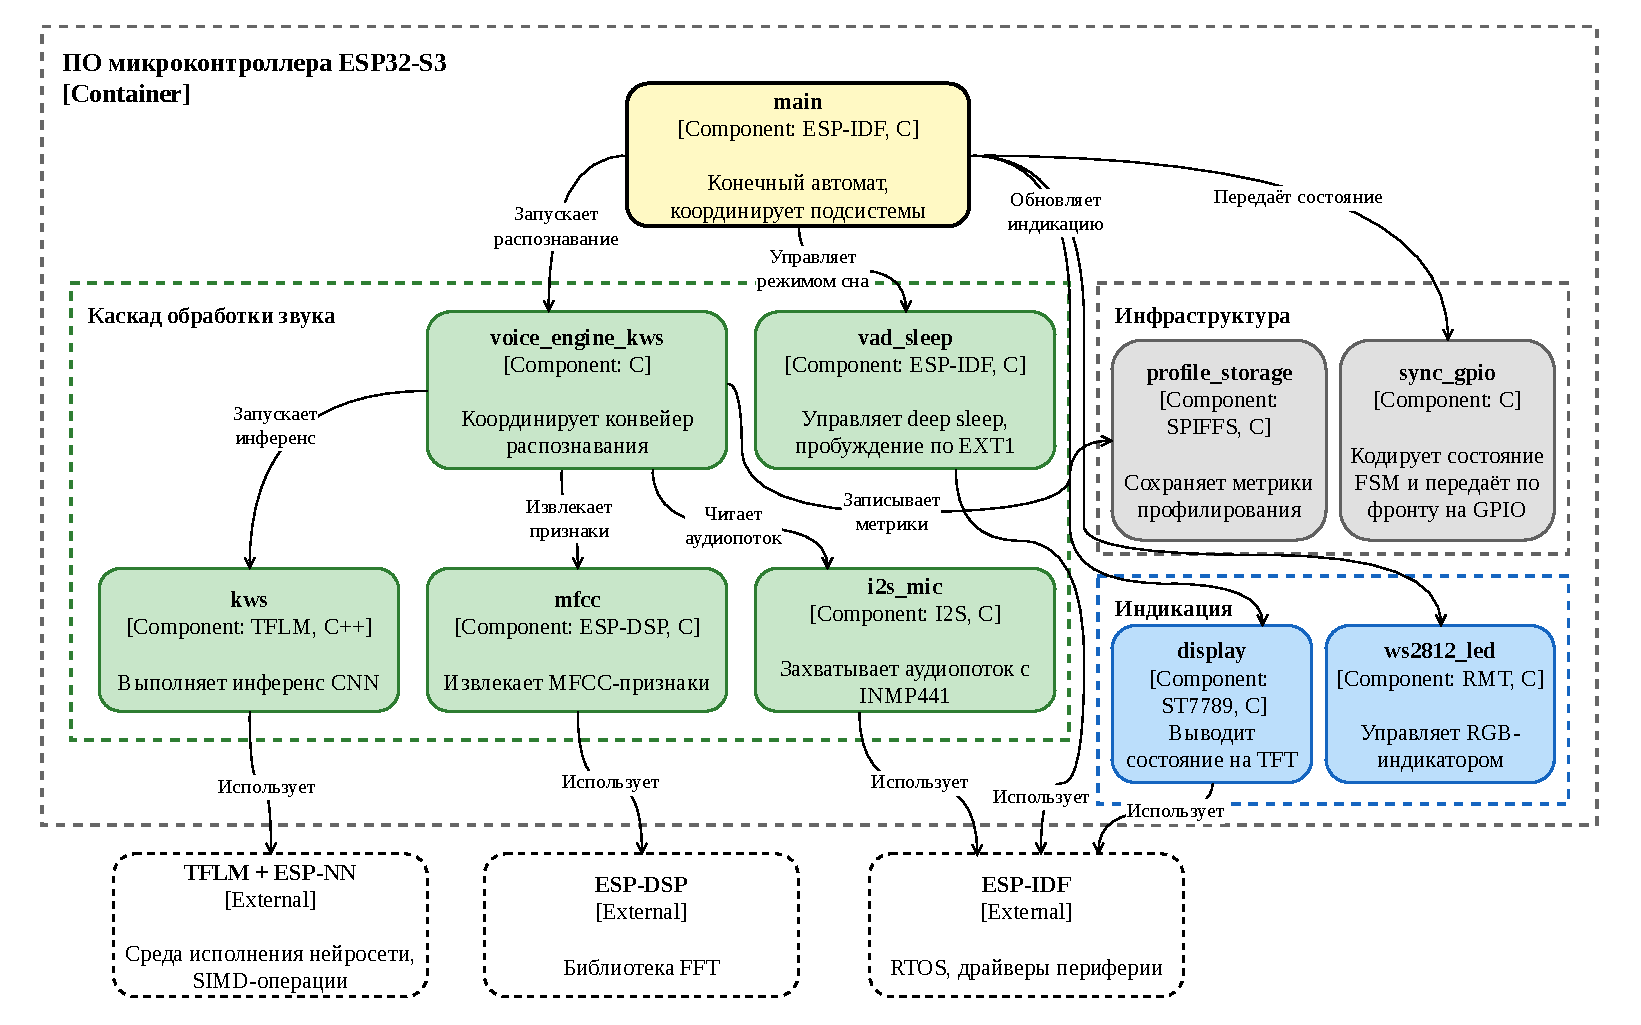
\includegraphics[width=1\textwidth]{assets/diagrams/software_c4_component_diagram.pdf}
	\caption{Компонентная диаграмма программной системы микроконтроллера в нотации C4}
	\label{fig:c4_components}
\end{figure}

Главный модуль \texttt{main.c} реализует оркестрацию состояний
конечного автомата; модуль \texttt{vad\_sleep} управляет
переходами в режим глубокого сна и обработкой пробуждения по
EXT1; модули \texttt{i2s\_mic}, \texttt{mfcc} и \texttt{kws}
реализуют соответственно захват аудиосигнала, извлечение
MFCC-признаков и инференс нейросетевой модели; модуль
\texttt{voice\_engine\_kws} объединяет компоненты пайплайна в
единый цикл обработки. Вспомогательные модули
\texttt{sync\_gpio}, \texttt{profile\_storage},
\texttt{display}, \texttt{st7789} и \texttt{ws2812\_led}
обеспечивают синхронизацию с измерительным стендом, локальное
хранение профилей и визуальную индикацию состояния системы. Все
модули опираются на стандартные подсистемы фреймворка ESP-IDF и
внешние библиотеки ESP-DSP (для аппаратно-ускоренных операций
БПФ), TensorFlow Lite Micro~\cite{src:4} и ESP-NN~\cite{src:9}
(для нейросетевого инференса).

Полный исходный код прошивки доступен в репозитории автора по
ссылке, приведённой в приложении~\ref{app:repos}. Ключевые
фрагменты, иллюстрирующие реализацию пробуждения по EXT1 и
конфигурации интерпретатора TensorFlow Lite Micro, приведены в
приложении~\ref{app:firmware_code}.

\subsubsection{Аппаратные регистры и режимы питания ESP32-S3}

Описание архитектуры доменов питания, регистров управления
энергосберегающими режимами и логики работы сопроцессора ULP, на
которые опирается реализация переходов между состояниями,
приведено в техническом справочнике на платформу~\cite{src:18}.
В режиме глубокого сна основные ядра Xtensa LX7, цифровая
периферия, модули Wi-Fi и Bluetooth обесточены; активными
остаются домен RTC и сопроцессор ULP. Согласно паспортным
характеристикам кристалла, потребление в данном режиме
составляет порядка 7--8~мкА~\cite{src:9}, тогда как фактическое
потребление модуля ESP32-S3-Zero, использованного в работе,
существенно выше из-за вклада компонентов обвязки; обсуждение
этого расхождения проводится в разделе~4.

\subsection{Реализация тракта обработки звука}

Тракт обработки звука ступени~2 каскада реализован программно на
основном ядре микроконтроллера и выполняется в состоянии
\texttt{MFCC} конечного автомата. Конкретные параметры
конвейера предобработки (частота дискретизации $f_s = 16$~кГц,
длительность фрейма $T_w = 40$~мс, шаг сегментации
$T_s = 20$~мс, число мел-фильтров $M = 40$ в диапазоне
20--4000~Гц, число сохраняемых кепстральных коэффициентов
$C = 10$) выбраны в соответствии с конфигурацией, основанной на
эталонной конфигурации Hello Edge~\cite{src:1}, и обоснованы в
разделе~2.

Полный конвейер предобработки от исходного звукового сигнала до
матрицы MFCC-признаков, подаваемой на вход нейросетевой модели,
представлен на рис.~\ref{fig:mfcc_pipeline} на примере одного
произнесения слова <<yes>>.

\begin{figure}[h!]
	\centering
	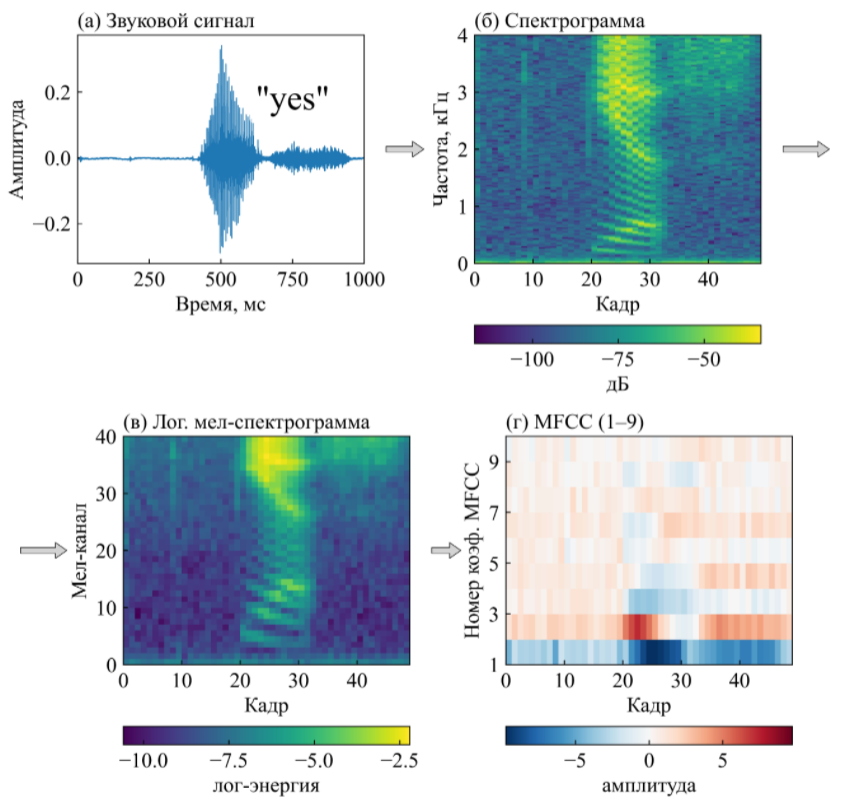
\includegraphics[width=0.9\textwidth]{assets/diagrams/feature_pipeline_improved_v2.png}
	\caption{Конвейер извлечения MFCC-признаков: исходный звуковой сигнал, его спектрограмма, логарифмическая мел-спектрограмма и итоговая матрица кепстральных коэффициентов}
	\label{fig:mfcc_pipeline}
\end{figure}

\subsubsection{Захват аудио}

Аудиосигнал поступает с цифрового MEMS-микрофона
INMP441~\cite{src:15} через аппаратный контроллер I2S
микроконтроллера в режиме Philips: разрядность слота 32~бита,
монорежим, частота дискретизации $f_s = 16$~кГц. Из 32-битного
представления полезные 18~бит АЦП микрофона расположены в
старших разрядах; приведение к 16-битному представлению
выполняется арифметическим сдвигом вправо на 14~разрядов, что
эквивалентно усечению младших разрядов шума. Захват выполняется
в кольцевой буфер DMA, что обеспечивает работу аудиотракта
параллельно с вычислительными задачами на основном ядре.

\subsubsection{Сегментация и оконная функция}

Одна секунда записи содержит $N = f_s \cdot 1\,\text{с} = 16000$
отсчётов. При длине фрейма в отсчётах $L = T_w \cdot f_s = 640$
и шаге $S = T_s \cdot f_s = 320$ количество фреймов в одной
секунде аудио составляет

\begin{equation}
	F = \left\lfloor \frac{N - L}{S} \right\rfloor + 1 = 49,
	\label{eq:frame_count}
\end{equation}

что в точности соответствует размерности входного тензора DS-CNN
($49 \times 10$), зафиксированной в разделе~2. К каждому фрейму
применяется оконная функция Хэмминга

\begin{equation}
	w[n] = 0{,}54 - 0{,}46 \cdot \cos\!\left(\frac{2 \pi n}{L - 1}\right),
	\quad n = 0, 1, \ldots, L-1,
	\label{eq:hamming}
\end{equation}

назначение которой~--- подавление спектральной утечки на
границах фрейма, неизбежной при прямоугольной сегментации
непрерывного сигнала. Выбор оконной функции Хэмминга (а не Ханна
или Блэкмана) обусловлен балансом между уровнем боковых
лепестков спектральной характеристики окна и шириной главного
лепестка, оптимальным для частотного разрешения речевых
формант.

\subsubsection{Дискретное преобразование Фурье}

Для приведения к ближайшей сверху степени двойки размер БПФ
выбран $N_{\mathrm{FFT}} = 1024$, отсчёты фрейма дополняются
нулями до этой длины. Разрешение БПФ по частоте составляет

\begin{equation}
	\Delta f = \frac{f_s}{N_{\mathrm{FFT}}} \approx 15{,}6~\text{Гц},
	\label{eq:fft_resolution}
\end{equation}

что обеспечивает достаточное частотное разрешение для разделения
формант речи в диапазоне до 4~кГц. БПФ реализуется через функцию
\texttt{dsps\_fft2r\_fc32} библиотеки ESP-DSP, оптимизированную
под векторные SIMD-инструкции архитектуры Xtensa LX7. Аппаратное
ускорение БПФ сокращает время выполнения данного этапа кратно по
сравнению со скалярной реализацией, что напрямую влияет на
длительность ступени~2 и, как следствие, на её вклад в
энергобюджет цикла.

\subsubsection{Мел-фильтрация, логарифмирование, ДКП}

Спектр мощности фрейма проецируется на $M = 40$ треугольных
мел-фильтров, равномерно распределённых по психоакустически
мотивированной мел-шкале

\begin{equation}
	\mathrm{mel}(f) = 2595 \cdot \log_{10}\!\left(1 + \frac{f}{700}\right),
	\label{eq:mel_scale}
\end{equation}

где $f$~--- циклическая частота в герцах. Использование
мел-шкалы вместо линейной отражает нелинейность восприятия
частоты человеческим слухом: разрешающая способность слуха выше
в низкочастотной области и снижается с ростом частоты, что
соответствует характеру речевого сигнала, в котором фонемоносная
информация сосредоточена в нижней части спектра.

К энергиям мел-фильтров применяется натуральный логарифм с
защитной аддитивной добавкой $\varepsilon = 10^{-10}$ для
исключения числовой неопределённости при нулевой энергии:

\begin{equation}
	E_m^{\log} = \ln\!\bigl(E_m + \varepsilon\bigr),
	\quad m = 1, 2, \ldots, M.
	\label{eq:log_mel}
\end{equation}

Логарифмирование выполняет двойную функцию: во-первых,
обеспечивает динамическое сжатие спектра, переводя громкость в
перцептивно-линейную шкалу (закон Вебера--Фехнера); во-вторых,
разделяет в кепстральной области свёрточные компоненты
сигнала~--- источник возбуждения и амплитудно-частотную
характеристику речевого тракта.

К вектору логарифмических энергий мел-фильтров применяется
дискретное косинусное преобразование II типа, из результата
которого сохраняются первые $C = 10$ коэффициентов:

\begin{equation}
	c_k = \sqrt{\frac{2}{M}} \sum_{m=1}^{M} E_m^{\log} \cdot
	\cos\!\left[ \frac{\pi k}{M} \left(m - \frac{1}{2}\right) \right],
	\quad k = 0, 1, \ldots, C-1.
	\label{eq:dct}
\end{equation}

Сохранение лишь первых десяти коэффициентов мотивировано тем,
что младшие кепстральные коэффициенты описывают грубую огибающую
спектра речевого тракта (формантную структуру), наиболее
информативную для задачи фонемной классификации, тогда как
старшие коэффициенты описывают мелкомасштабные спектральные
детали, связанные преимущественно с источником возбуждения и
индивидуальными особенностями диктора. Аналогичный принцип
отсечения коэффициентов экспериментально обоснован в смежной
задаче снижения размерности признакового пространства для
распознавания речевых эмоций в работе Исхаковой и
др.~\cite{src:26}.

Результирующая матрица $49 \times 10$ образует входной тензор
DS-CNN. На рис.~\ref{fig:mfcc_words} приведены примеры
MFCC-матриц для четырёх ключевых слов из набора Google Speech
Commands. Визуально различимая кепстральная структура для
разных классов команд подтверждает, что выбранное признаковое
пространство сохраняет информацию, необходимую для
последующей классификации; одновременно близость кепстральных
паттернов внутри пар акустически близких слов
(<<no>>/<<go>>) объясняет характер ошибок классификатора,
рассматриваемых в разделе~4.

\begin{figure}[h!]
	\centering
	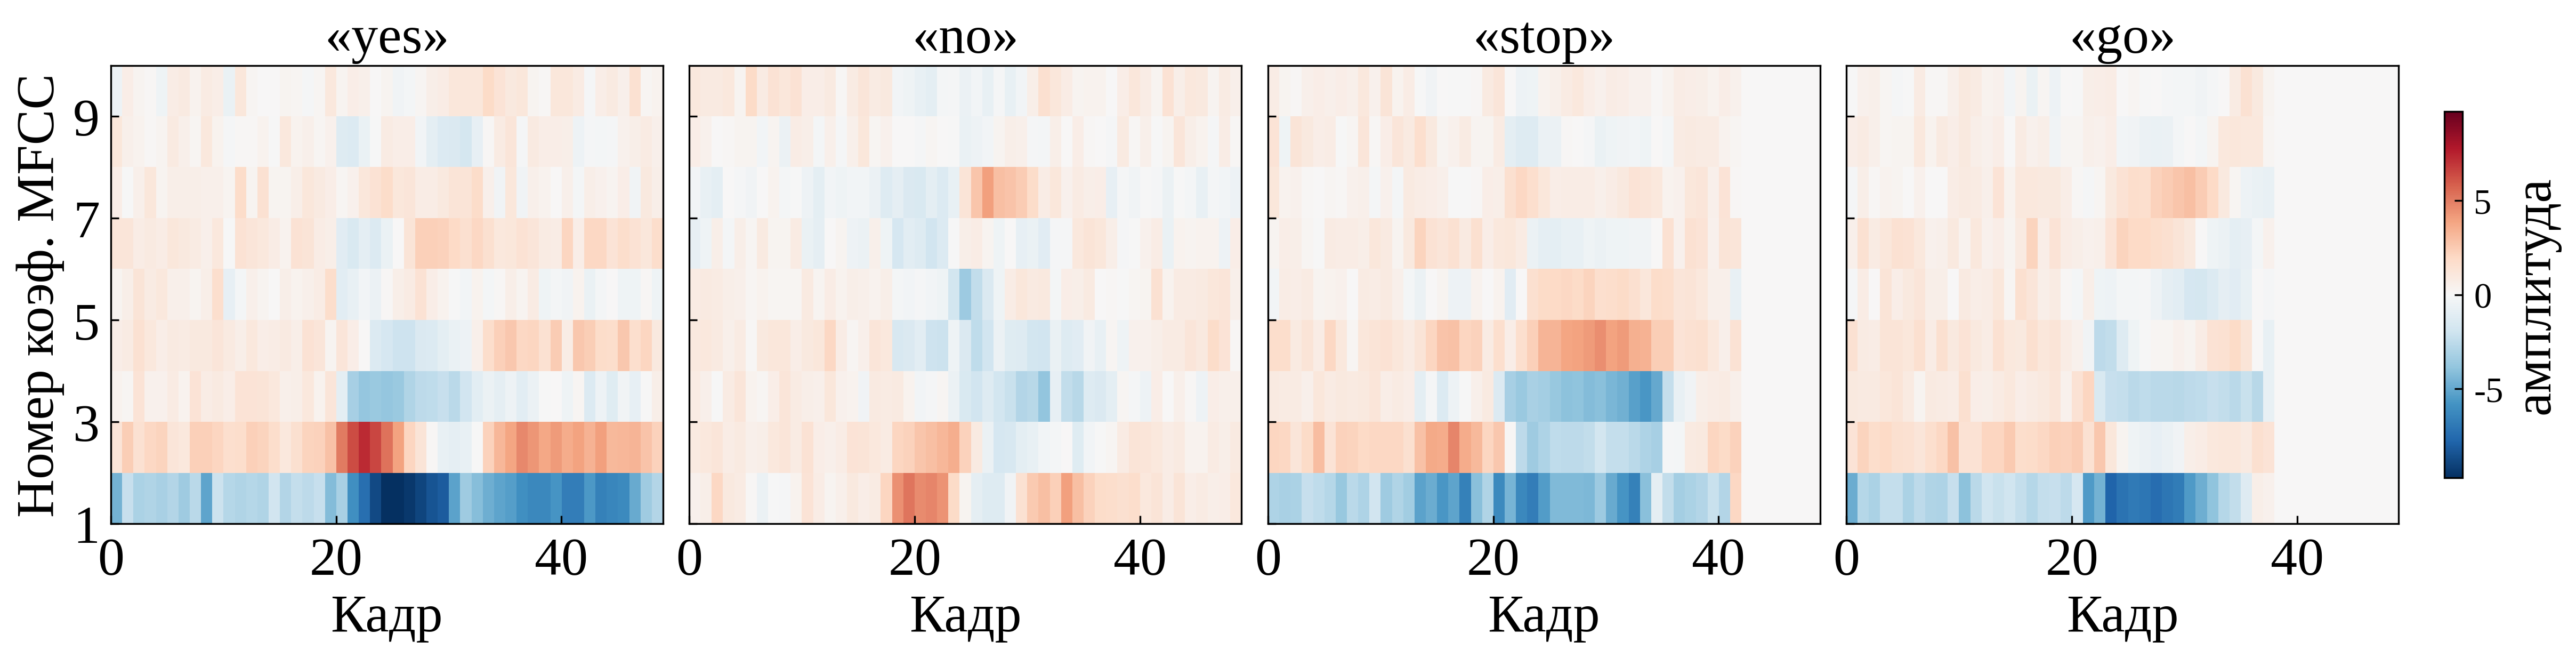
\includegraphics[width=1\textwidth]{assets/diagrams/mfcc_words_improved_v2.png}
	\caption{Матрицы MFCC-признаков для четырёх ключевых слов из набора Google Speech Commands: <<yes>>, <<no>>, <<stop>>, <<go>>}
	\label{fig:mfcc_words}
\end{figure}

\subsection{Реализация инференса нейросетевой модели}

Инференс квантизованной модели DS-CNN выполняется на основном
ядре ESP32-S3 фреймворком TensorFlow Lite Micro~\cite{src:4} с
аппаратным ускорением через библиотеку ESP-NN, реализующую ядра
свёрточных операций на SIMD-инструкциях Xtensa~LX7.

Инициализация интерпретатора TFLM включает три этапа. Первый~---
загрузка модели из массива \texttt{g\_model\_data},
размещённого во флеш-памяти и получаемого экспортом обученной
модели в формат \texttt{.tflite} с последующим преобразованием в
массив \texttt{const uint8\_t}. Второй~--- регистрация
используемых операторов в регистраторе операторов
(op-resolver): \texttt{Conv2D}, \texttt{DepthwiseConv2D},
\texttt{FullyConnected}, \texttt{Mean} (для глобального
усреднения), \texttt{Reshape}, \texttt{Quantize},
\texttt{Dequantize} и \texttt{Softmax}. Третий~--- аллокация
арены тензоров, статически выделяемой области оперативной
памяти, используемой TFLM для размещения промежуточных
тензоров без динамической аллокации.

В реализации настоящей работы арена тензоров размером 140~КБ
располагается во внутреннем SRAM микроконтроллера (а не во
внешней PSRAM), поскольку аппаратное SIMD-ускорение библиотеки
ESP-NN корректно работает только с памятью, физически доступной
по шине внутреннего SRAM.

Подача данных на вход интерпретатора требует квантизации
матрицы MFCC-признаков из формата FP32 в формат INT8 с
использованием масштабного коэффициента и нулевой точки,
считанных из метаданных входного тензора модели, согласно
формуле~(2.2) раздела~2. После выполнения инференса (вызов
\texttt{Interpreter::Invoke()}) выходной вектор логитов в
формате INT8 деквантизуется обратно в вещественные значения, и
в качестве решения классификатора выбирается класс с
максимальным значением логита. Ключевой фрагмент кода
инференса приведён в приложении~\ref{app:firmware_code}, полный
код~--- в репозитории прошивки
(приложение~\ref{app:repos}).

\subsection{Методика исследования пространства архитектур}

В разделе~2 в качестве класса нейросетевого классификатора
выбрана архитектура DS-CNN; конкретные значения гиперпараметров
определяются по результатам систематического экспериментального
исследования, методика которого описана в настоящем подразделе.

\subsubsection{Сетка обучаемых архитектур}

Семейство архитектур DS-CNN определяется двумя ключевыми
гиперпараметрами: числом фильтров в свёрточных слоях $F$ и
числом блоков разделимой свёртки $B$. Для систематического
исследования зависимости точности классификации от этих
параметров обучено множество моделей, образующих
прямоугольную сетку в пространстве $(F, B)$:

\begin{itemize}
	\item значения $F$: 16, 24, 32, 40, 48, 56, 64, 72, 80, 88,
	      96, 104, 112, 128, 160, 168, 172, 176, 184, 192, 224
	      (всего 21 значение, шаг 8 в основном диапазоне);
	\item значения $B$: 2, 3, 4, 5, 6, 7, 8 (всего 7 значений).
\end{itemize}

Диапазон $F$ выбран с шагом 8, кратным размеру SIMD-регистра
архитектуры Xtensa LX7 (128~бит, что соответствует 16 элементам
INT8 для весов pointwise-свёрток). Базовое значение $F=172$
эталонной конфигурации Hello Edge~\cite{src:1} \emph{не} кратно
8 и сохранено в сетке как референсная точка для сопоставления
с литературой. Диапазон $B$ от~2 до~8 охватывает мелкие
архитектуры с минимальной глубиной до моделей, в полтора раза
более глубоких, чем эталонная (где $B=6$).

Из полной декартовой сетки исключены архитектуры с
очевидно недостаточной ёмкостью ($F=16, B=2$~--- менее 2000
параметров) и архитектуры, которые в предварительных запусках
демонстрировали расходимость обучения. Итоговое число обученных
архитектур составило 134.

\subsubsection{Методика обучения}

Все архитектуры обучены по единой методике, описанной в
разделе~3.4 (приведена ниже в подразделе~3.4.3 для удобства
изложения). Общий конвейер обучения и квантизации представлен
на рис.~\ref{fig:training_pipeline}: набор Google Speech
Commands~v2~\cite{src:2} разделяется на обучающую, валидационную
и тестовую выборки в соотношении 80:10:10 при условии, что
записи одного диктора попадают только в одну из выборок.

\begin{figure}[H]
	\centering
	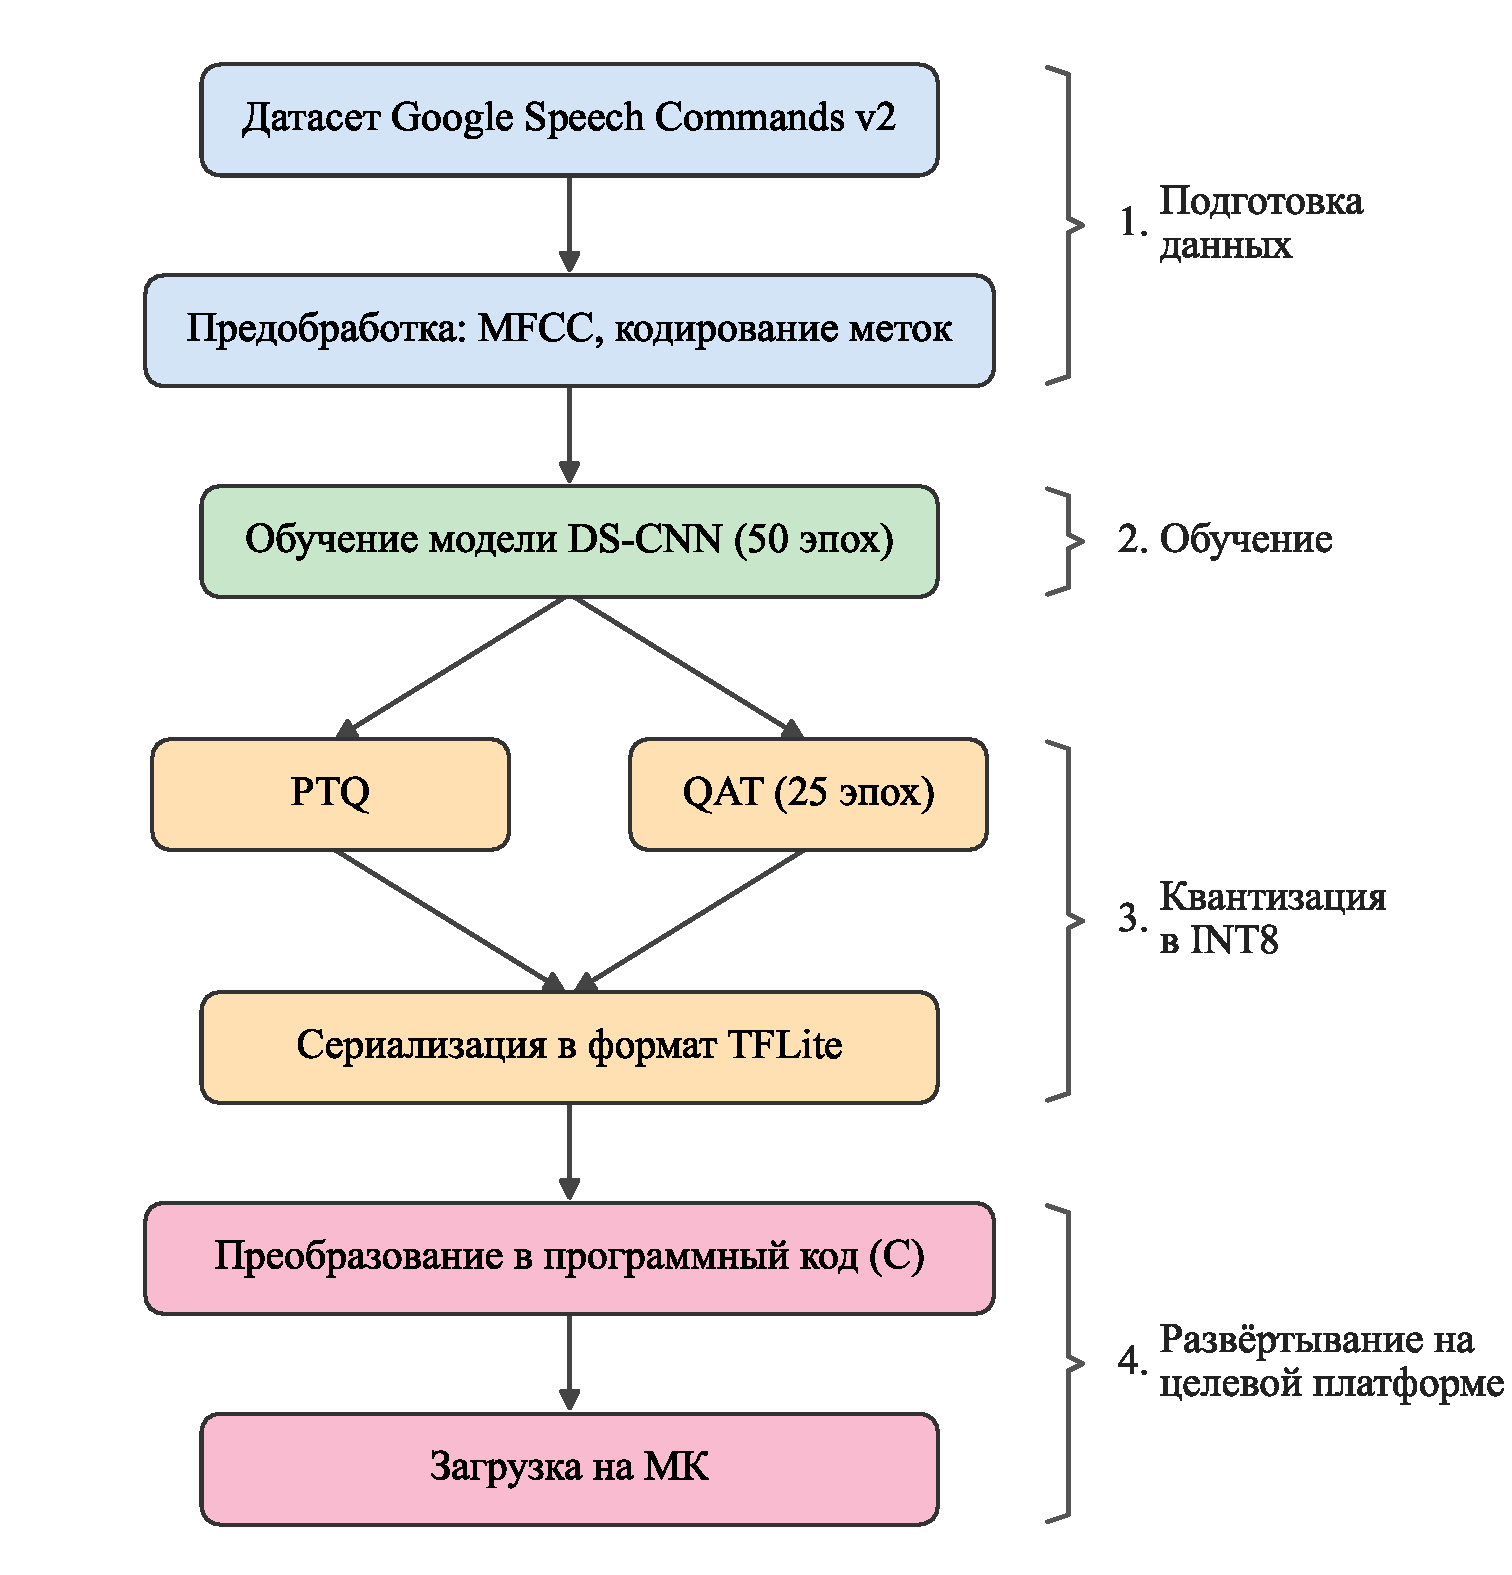
\includegraphics[width=1\textwidth]{assets/diagrams/training_pipeline.pdf}
	\caption{Конвейер обучения и квантизации нейросетевой модели}
	\label{fig:training_pipeline}
\end{figure}

Каждая FP32-модель обучается в течение 50 эпох оптимизатором
Adam с косинусным расписанием снижения скорости обучения от
$10^{-3}$ до $10^{-5}$, размером мини-батча 100, функцией
потерь~--- категориальной перекрёстной энтропией с применением
сглаживания меток (label smoothing, коэффициент 0,1).
Аугментация обучающих данных включает случайный временно\'{й}
сдвиг произнесения в пределах $\pm$100~мс и наложение фоновых
шумов из набора Speech Commands.

Для каждой архитектуры выполняется квантизация обученной
FP32-модели методом PTQ, а для подмножества архитектур
(105~моделей) дополнительно методом QAT с дообучением на
протяжении 25~эпох с пониженной скоростью обучения $10^{-4}$.
Тем самым общее число оцениваемых вариантов в исследовании
составляет 239 точек (134~FP32, 134~PTQ, 105~QAT).

Полные исходные тексты модулей обучения и квантизации
приведены в приложении~\ref{app:python_code}; ключевые
фрагменты~--- архитектура \texttt{ds\_cnn.py}, цикл обучения
\texttt{train.py}, конвертация PTQ и QAT~--- доступны в
репозитории автора (приложение~\ref{app:repos}).

\subsubsection{Метрики и статистическая значимость}

Для каждой архитектуры в исследовании сохраняются: точность
классификации FP32-модели и каждой из квантизованных моделей
на тестовой выборке; размер итогового файла \texttt{.tflite};
число параметров модели; время обучения; служебные метаданные
(дата обучения, конфигурация, флаг SIMD-выравнивания).

Тестовая выборка Google Speech Commands~v2 содержит
$n_{\mathrm{test}} = 4154$~образца. Точность классификации на
выборке такого размера измеряется с конечной статистической
погрешностью. Доверительный интервал точности рассчитывается по
формуле Уилсона для биномиальной пропорции~\cite{src:32}:

\begin{equation}
	p \in \left[
		\frac{\hat{p} + \frac{z^2}{2n} - z\sqrt{\frac{\hat{p}(1-\hat{p})}{n} + \frac{z^2}{4n^2}}}{1 + \frac{z^2}{n}};\,
		\frac{\hat{p} + \frac{z^2}{2n} + z\sqrt{\frac{\hat{p}(1-\hat{p})}{n} + \frac{z^2}{4n^2}}}{1 + \frac{z^2}{n}}
		\right],
	\label{eq:wilson}
\end{equation}

где $\hat{p}$~--- наблюдаемая доля верных классификаций;
$n$~--- объём тестовой выборки; $z$~--- критическое значение
стандартного нормального распределения для заданного уровня
доверия. Для уровня 95\% ($z \approx 1{,}96$) и
$\hat{p} \approx 0{,}95$, $n = 4154$, ширина доверительного
интервала составляет приблизительно $\pm 0{,}65$~п.п. Различия
в точности между моделями, не превышающие указанной величины,
не являются статистически значимыми и в дальнейшем
интерпретируются как шум.

Графическое представление результатов обучения всей сетки
архитектур, а также Парето-граница в координатах (точность,
размер модели INT8), составляют содержание подраздела~4.1.

\subsection{Лабораторный измерительный стенд}

Для количественной оценки энергопотребления каскадной системы
разработан двухдоменный лабораторный стенд, изолирующий
измеряемую систему и систему измерений в независимые
электрические домены. Подобное разделение обеспечивает
корректную регистрацию потребления в диапазоне от единиц
микроампер (в режиме глубокого сна) до сотен миллиампер (при
активном инференсе) без внесения паразитных токов системы
измерений в шину питания исследуемой платы. Принципиальная схема
стенда приведена в приложении~\ref{app:schematic}, общий
вид~--- в приложении~\ref{app:photos}, диаграмма
последовательности сбора данных~--- на
рис.~\ref{fig:sequence_diagram}.

\subsubsection{Домен~1: измеряемая система}

Домен~1 включает компоненты, потребление которых является
объектом измерения, и питается от литий-ионного
аккумулятора~18650 номинальным напряжением 3,7~В и ёмкостью
2600~мА$\cdot$ч с модулем защиты и зарядки TP4056. Состав
домена:

\begin{itemize}
	\item микроконтроллер: модуль на базе ESP32-S3 с 8~МБ
	      флеш-памяти и 8~МБ внешней PSRAM, выведенными на разъёмы
	      11~пользовательскими GPIO, из которых пять поддерживают
	      функцию RTC GPIO и могут быть использованы как
	      источники пробуждения EXT0/EXT1 из режима глубокого
	      сна;
	\item микрофон: цифровой MEMS-микрофон INMP441 производства
	      InvenSense (TDK)~\cite{src:15} с интерфейсом I2S,
	      отношением сигнал/шум 61~дБА, динамическим диапазоном
	      87~дБ, частотным диапазоном 60~Гц~--- 15~кГц и типовым
	      потреблением 1,4~мА в активном режиме при напряжении
	      питания 3,3~В;
	\item детектор звука первой ступени каскада: модуль на базе
	      компаратора LM393 с электретным микрофонным капсюлем и
	      подстроечным резистором настройки порога; выход
	      подключён к выводу RTC GPIO микроконтроллера для
	      пробуждения по EXT1;
	\item индикация результата: светодиод, подключённый к
	      выводу RTC GPIO для визуальной индикации обнаруженной
	      команды;
	\item дисплей: TFT-дисплей на базе контроллера ST7789,
	      подключённый по SPI, для отображения состояния системы
	      и результата классификации в режиме отладки.
\end{itemize}

Между аккумулятором и шиной питания домена~1 в разрыв включён
датчик тока и мощности~--- микросхема Texas Instruments INA228
в качестве чувствительного элемента стенда.

\subsubsection{Датчик тока INA228}

INA228~\cite{src:16} представляет собой монитор мощности с
20-битным сигма-дельта-АЦП, диапазоном измерения тока от единиц
микроампер до сотен миллиампер и интерфейсом I2C. В стенде
использован шунтовой резистор $R_{\mathrm{sh}} = 100$~мОм,
включённый в разрыв линии питания между аккумулятором и шиной
домена~1. Согласно документации производителя~\cite{src:16},
наименьший значащий разряд канала измерения напряжения на
шунте составляет 312,5~нВ, что при $R_{\mathrm{sh}} = 100$~мОм
соответствует разрешению по току на уровне единиц
микроампер~--- величине, необходимой для регистрации
потребления в режиме глубокого сна.

Калибровочный регистр \texttt{SHUNT\_CAL} датчика
программируется согласно методике
производителя~\cite{src:16} исходя из выбранного сопротивления
шунта $R_{\mathrm{sh}}$ и максимального ожидаемого тока
$I_{\max}$:

\begin{equation}
	\mathrm{CURRENT\_LSB} = \frac{I_{\max}}{2^{19}},
	\label{eq:current_lsb}
\end{equation}

\begin{equation}
	\mathrm{SHUNT\_CAL} = 13107200 \cdot \mathrm{CURRENT\_LSB} \cdot R_{\mathrm{sh}},
	\label{eq:shunt_cal}
\end{equation}

где $\mathrm{CURRENT\_LSB}$~--- наименьший значащий разряд
канала тока в амперах; $I_{\max}$~--- максимальный ожидаемый
ток в амперах; $R_{\mathrm{sh}}$~--- сопротивление шунта в
омах; числовой множитель $13{,}1072 \cdot 10^{6}$~---
внутренняя константа АЦП INA228 в режиме
\texttt{ADCRANGE = 0}. Для условий настоящей работы выбраны
$R_{\mathrm{sh}} = 0{,}1$~Ом и $I_{\max} = 0{,}5$~А, что даёт
$\mathrm{CURRENT\_LSB} \approx 0{,}954$~мкА на отсчёт и
охватывает диапазон от глубокого сна до пиков активного
инференса с запасом.

Период опроса регистров INA228 (\texttt{VBUS},
\texttt{CURRENT}, \texttt{VSHUNT}) выбран равным 200~мс.
Обоснование выбора периода приведено в подразделе~3.7. Данные
передаются логгеру по шине~I2C.

\subsubsection{Домен~2: система измерений (логгер)}

Домен~2 питается от отдельного аккумулятора 18650 и
электрически изолирован от домена~1; токи, потребляемые
компонентами домена~2, не влияют на показания INA228. Состав
домена:

\begin{itemize}
	\item микроконтроллер логгера: ESP32-C3 Mini~---
	      одноядерный процессор RISC-V с тактовой частотой
	      160~МГц; через шину I2C опрашивает регистры INA228 с
	      периодом 200~мс;
	\item канал передачи данных: USB-UART-мост, через который
	      логгер транслирует пакеты измерений на персональный
	      компьютер в формате CSV со столбцами
	      \texttt{timestamp}, \texttt{bus\_v},
	      \texttt{current\_ma}, \texttt{shunt\_uv},
	      \texttt{power\_mw}, а также два бита состояния FSM,
	      опрашиваемые через дополнительные GPIO для
	      синхронизации с этапами обработки;
	\item постобработка: Python-скрипт на ПК принимает CSV-поток,
	      строит профили мгновенного тока и сохраняет данные для
	      последующего анализа.
\end{itemize}

Диаграмма последовательности сбора измерительных данных
приведена на рис.~\ref{fig:sequence_diagram}: микроконтроллер
ESP32-S3 кодирует состояние FSM на двух выводах GPIO; логгер
ESP32-C3 параллельно опрашивает эти GPIO и читает регистры
INA228 по I2C; результаты передаются на ПК через USB-UART в
виде CSV-пакетов.

\begin{figure}[h!]
	\centering
	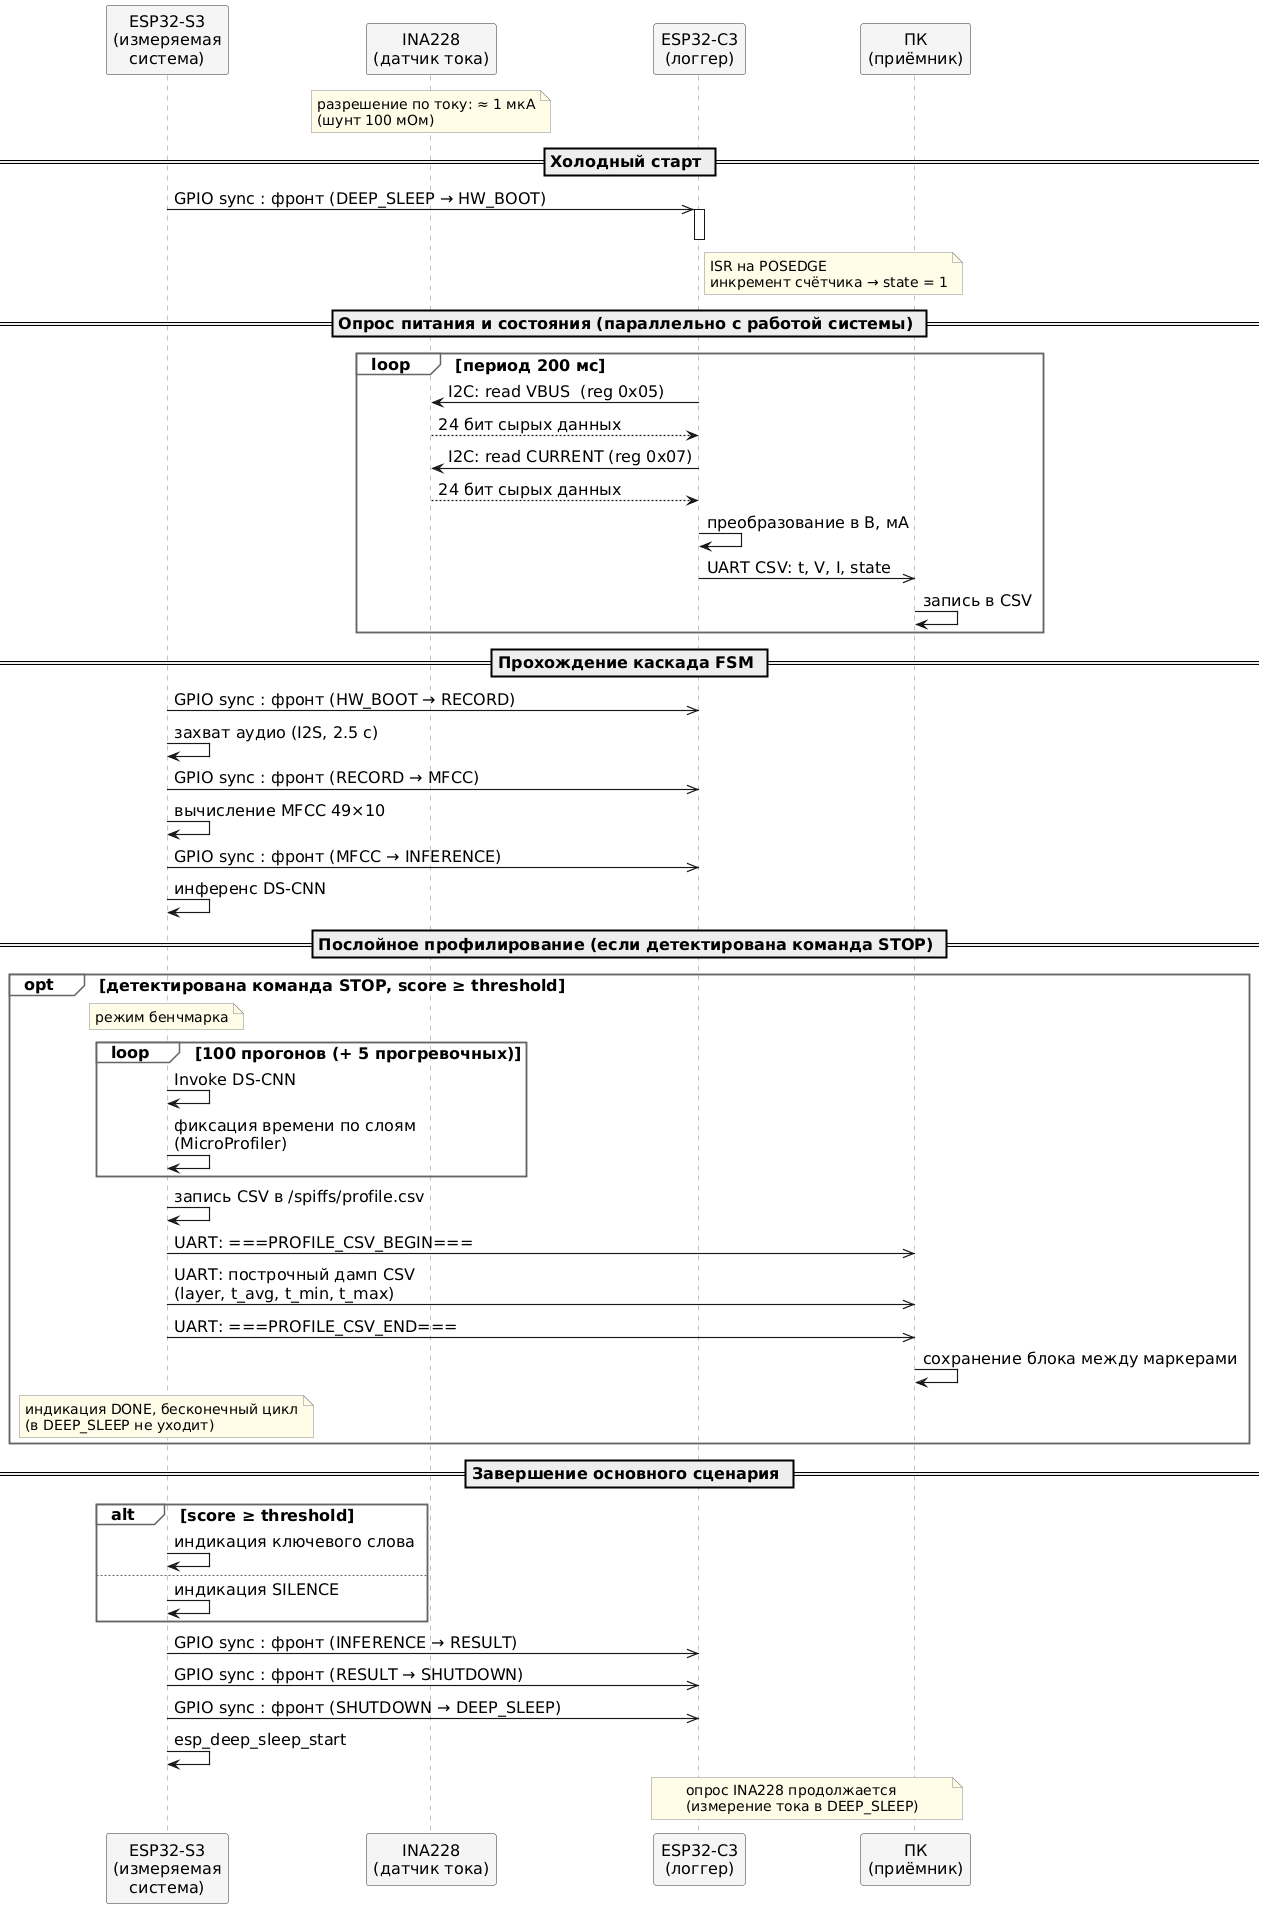
\includegraphics[width=1\textwidth]{assets/diagrams/measurements_sequence_diagram.png}
	\caption{Диаграмма последовательности сбора измерительных данных}
	\label{fig:sequence_diagram}
\end{figure}

Принципиальная схема разделения доменов и подключения
компонентов приведена в приложении~\ref{app:schematic};
фотография собранного стенда~--- в приложении~\ref{app:photos}.

\subsection{Методика экспериментальной апробации}

Методика эксперимента определяется задачами, поставленными в
разделе~1: охарактеризовать предложенную каскадную архитектуру
по совокупности заявленных метрик (точность классификации,
средняя потребляемая мощность, энергия на детекцию, время
инференса, размер модели) и выполнить декомпозицию энергобюджета
каскадного цикла по этапам обработки. Эксперимент состоит из
двух последовательных частей.

\subsubsection{Характеризация моделей в программной среде}

В программной среде (TensorFlow~2 на персональном компьютере)
для каждой из 134~обученных архитектур измеряются: итоговая
точность классификации FP32-модели на тестовой выборке Google
Speech Commands; точность каждой из квантизованных моделей
(PTQ INT8 и, где применимо, QAT INT8), получаемая запуском
квантизованной модели на той же тестовой выборке через
интерпретатор TensorFlow Lite на центральном процессоре; размер
итоговых файлов \texttt{.tflite}; число параметров. Результаты
этой части эксперимента приведены в разделе~4 (подразделы 4.1
и~4.2).

\subsubsection{Характеризация системы на платформе ESP32-S3}

На платформе ESP32-S3 с собранным измерительным стендом для
подмножества архитектур из Парето-границы (отбор которого
обоснован в разделе~4) измеряются: профиль мгновенного тока
полного цикла каскадной обработки от пробуждения по EXT1 до
возврата в режим глубокого сна; время выполнения ступени~3
каскада (инференс через TFLM с ESP-NN), измеренное программно
через \texttt{esp\_timer\_get\_time()}; потребление системы в
режиме глубокого сна, измеренное на протяжении длительного
интервала наблюдения для усреднения шумов.

Для корреляции профиля потребления с состояниями конечного
автомата используется синхронизация через GPIO, описанная в
подразделе~3.1: два вывода микроконтроллера кодируют текущее
состояние FSM и опрашиваются логгером одновременно с
показаниями INA228. В постобработке участки CSV-файла,
соответствующие каждому состоянию FSM, выделяются автоматически
и обрабатываются раздельно. Результаты этой части эксперимента
приведены в разделе~4 (подразделы 4.3--4.6).

\subsubsection{Формулы обработки измерений}

Энергия, расходуемая на одно полное прохождение цикла каскадной
обработки, вычисляется численным интегрированием мгновенной
мощности по времени цикла. На промежутках между двумя
последовательными измерениями ($\Delta t = 200$~мс) мощность
считается постоянной, что соответствует приближению
прямоугольных импульсов:

\begin{equation}
	E_{\mathrm{cycle}} =
	\int_{t_0}^{t_1} P(t)\, dt \approx
	\sum_{k} P_k \cdot \Delta t,
	\label{eq:energy_cycle}
\end{equation}

где $E_{\mathrm{cycle}}$~--- энергия одного цикла в джоулях;
$P_k$~--- мгновенная мощность, зарегистрированная INA228 в
$k$-м отсчёте, в ваттах; $\Delta t = 0{,}2$~с~--- период
опроса. Энергобюджет цикла далее декомпозируется по этапам
обработки разбиением суммы~\eqref{eq:energy_cycle} на участки,
соответствующие отдельным состояниям FSM, что и составляет
содержание задачи декомпозиции, поставленной в разделе~1.

Энергия одного нейросетевого инференса, выделяемая в отдельную
метрику для сопоставления моделей различной архитектуры,
рассчитывается как

\begin{equation}
	E_{\mathrm{inf}} = \bar{I}_{\mathrm{INFERENCE}} \cdot
	\bar{V} \cdot t_{\mathrm{inf}},
	\label{eq:energy_inf}
\end{equation}

где $\bar{I}_{\mathrm{INFERENCE}}$~--- средний ток в состоянии
\texttt{INFERENCE} (в амперах); $\bar{V}$~--- среднее напряжение
на шине питания (в вольтах); $t_{\mathrm{inf}}$~--- длительность
инференса (в секундах).

Согласно модели~(2.1) раздела~2, средняя потребляемая мощность
системы определяется выражением

\begin{equation}
	\bar{P} = P_{\mathrm{sleep}} + f_{\mathrm{event}} \cdot E_{\mathrm{cycle}},
	\label{eq:avg_power_v2}
\end{equation}

где $\bar{P}$~--- средняя потребляемая мощность системы в
ваттах; $P_{\mathrm{sleep}}$~--- мощность в режиме глубокого
сна; $f_{\mathrm{event}}$~--- ожидаемая частота голосовых
событий (число пробуждений каскада в секунду).
Формула~\eqref{eq:avg_power_v2} представляет собой частный
случай формулы~(2.1) для трёхступенчатого каскада, в котором
ступени~2 и~3 объединены в одно состояние полного рабочего
цикла и активны только при срабатывании ступени~1.

Расчётное время автономной работы устройства от батареи
ёмкостью~$C$ оценивается из соотношения

\begin{equation}
	T_{\mathrm{auto}} = \frac{C}{\bar{I}},
	\label{eq:auto_time}
\end{equation}

где $T_{\mathrm{auto}}$~--- время непрерывной работы в часах;
$C$~--- ёмкость аккумулятора в миллиампер-часах; $\bar{I}$~---
средний ток потребления системы в миллиамперах, рассчитанный из
$\bar{P}$ и номинального напряжения питания.
Формула~\eqref{eq:auto_time} используется в разделе~4 для
пересчёта экспериментально измеренных значений $\bar{P}$ в
производный показатель, имеющий прямое практическое значение для
оценки применимости системы.

\subsubsection{Обоснование выбора периода опроса 200~мс}

Период опроса регистров INA228, равный 200~мс, выбран как
компромисс между двумя противоположными требованиями. Меньший
период позволил бы разрешить более короткие переходные
процессы, однако привёл бы к существенному увеличению объёма
CSV-файла и нагрузке на канал передачи данных USB-UART,
ограниченный пропускной способностью 115\,200~бод. Бо\'{л}ьший
период увеличил бы погрешность интегрирования энергии на
коротких этапах каскада (в первую очередь на этапе \texttt{MFCC}
длительностью порядка сотен миллисекунд).

При выбранном периоде 200~мс на каждом из основных этапов
каскада (длительностью от 500~мс до 3~с) укладывается от трёх до
пятнадцати отсчётов, что обеспечивает приемлемую точность
интегрирования энергии методом прямоугольных импульсов.
Внутреннее усреднение INA228 на окне $\approx 4{,}2$~мс
сглаживает короткие пики переходных процессов, а энергия
микросекундных переходов между состояниями пренебрежимо мала на
фоне многосекундных рабочих этапов. Тем самым выбранный период
обеспечивает корректную интегральную оценку энергобюджета цикла
при сохранении приемлемого объёма данных.

\subsection{Выводы по разделу}

В настоящем разделе описана практическая реализация каскадной
KWS-системы на платформе ESP32-S3, методика систематического
исследования архитектур нейросетевого классификатора и методика
экспериментальной апробации. Получены следующие результаты.

\begin{enumerate}
	\item Реализован конечный автомат каскада из семи состояний
	      с аппаратно-программной синхронизацией через GPIO,
	      обеспечивающей возможность раздельного измерения
	      энергопотребления каждого этапа цикла обработки.
	      Реализация выполнена средствами фреймворка ESP-IDF;
	      программная архитектура декомпозирована на независимые
	      модули в соответствии с компонентной диаграммой
	      рис.~\ref{fig:c4_components};
	\item Реализован тракт обработки звука ступени~2 каскада,
	      включающий захват аудиосигнала через I2S с цифрового
	      MEMS-микрофона INMP441, сегментацию сигнала на фреймы
	      по 40~мс с шагом 20~мс, применение оконной функции
	      Хэмминга, дискретное преобразование Фурье размером
	      1024~точки с аппаратным ускорением библиотеки ESP-DSP,
	      проекцию на 40~треугольных мел-фильтров,
	      логарифмирование и дискретное косинусное преобразование
	      с сохранением 10~кепстральных коэффициентов
	      (рис.~\ref{fig:mfcc_pipeline});
	\item Реализован инференс квантизованной модели DS-CNN через
	      фреймворк TensorFlow Lite Micro с аппаратным ускорением
	      библиотеки ESP-NN. Арена тензоров размером 140~КБ
	      размещена во внутреннем SRAM микроконтроллера для
	      обеспечения корректной работы SIMD-ускорения;
	\item Выполнено систематическое исследование пространства
	      архитектур DS-CNN: обучено 134~архитектуры в сетке
	      $F \in \{16, \ldots, 224\}$, $B \in \{2, \ldots, 8\}$,
	      для каждой выполнена квантизация PTQ, для
	      105~архитектур дополнительно QAT, итого получено
	      239~оцениваемых вариантов
	      (рис.~\ref{fig:heatmap_filters_blocks},
	      \ref{fig:pareto_size_acc});
	\item Сформулирована методика статистической оценки
	      точности с использованием доверительного интервала
	      Уилсона~\eqref{eq:wilson}, обеспечивающая
	      содержательную интерпретацию различий между моделями;
	\item Разработан двухдоменный лабораторный измерительный
	      стенд (приложения~\ref{app:schematic},
	      \ref{app:photos}), изолирующий измеряемую систему и
	      систему измерений в независимые электрические домены. В
	      качестве чувствительного элемента использован монитор
	      мощности INA228 с шунтом 100~мОм, обеспечивающий
	      разрешение по току на уровне единиц микроампер и
	      пригодный для регистрации потребления от глубокого сна
	      до пиков активного инференса;
	\item Сформулирована методика экспериментальной апробации,
	      включающая характеризацию моделей в программной среде
	      и характеризацию системы на платформе ESP32-S3, а также
	      приведены формулы обработки экспериментальных
	      данных~--- расчёта энергии цикла методом численного
	      интегрирования~\eqref{eq:energy_cycle}, расчёта энергии
	      одного инференса~\eqref{eq:energy_inf}, оценки средней
	      потребляемой мощности~\eqref{eq:avg_power_v2} и
	      расчётного времени автономной работы~\eqref{eq:auto_time}.
\end{enumerate}

Результаты применения описанной методики и интерпретация
полученных данных составляют содержание следующего раздела.
